%---------------------------------------------------------------------------%
%->> Section 3.4: SOP驱动的多智能体在线故障诊断方法
%---------------------------------------------------------------------------%

\section{SOP驱动的多智能体在线故障诊断方法}

\begin{figure}[htbp]
    \centering
    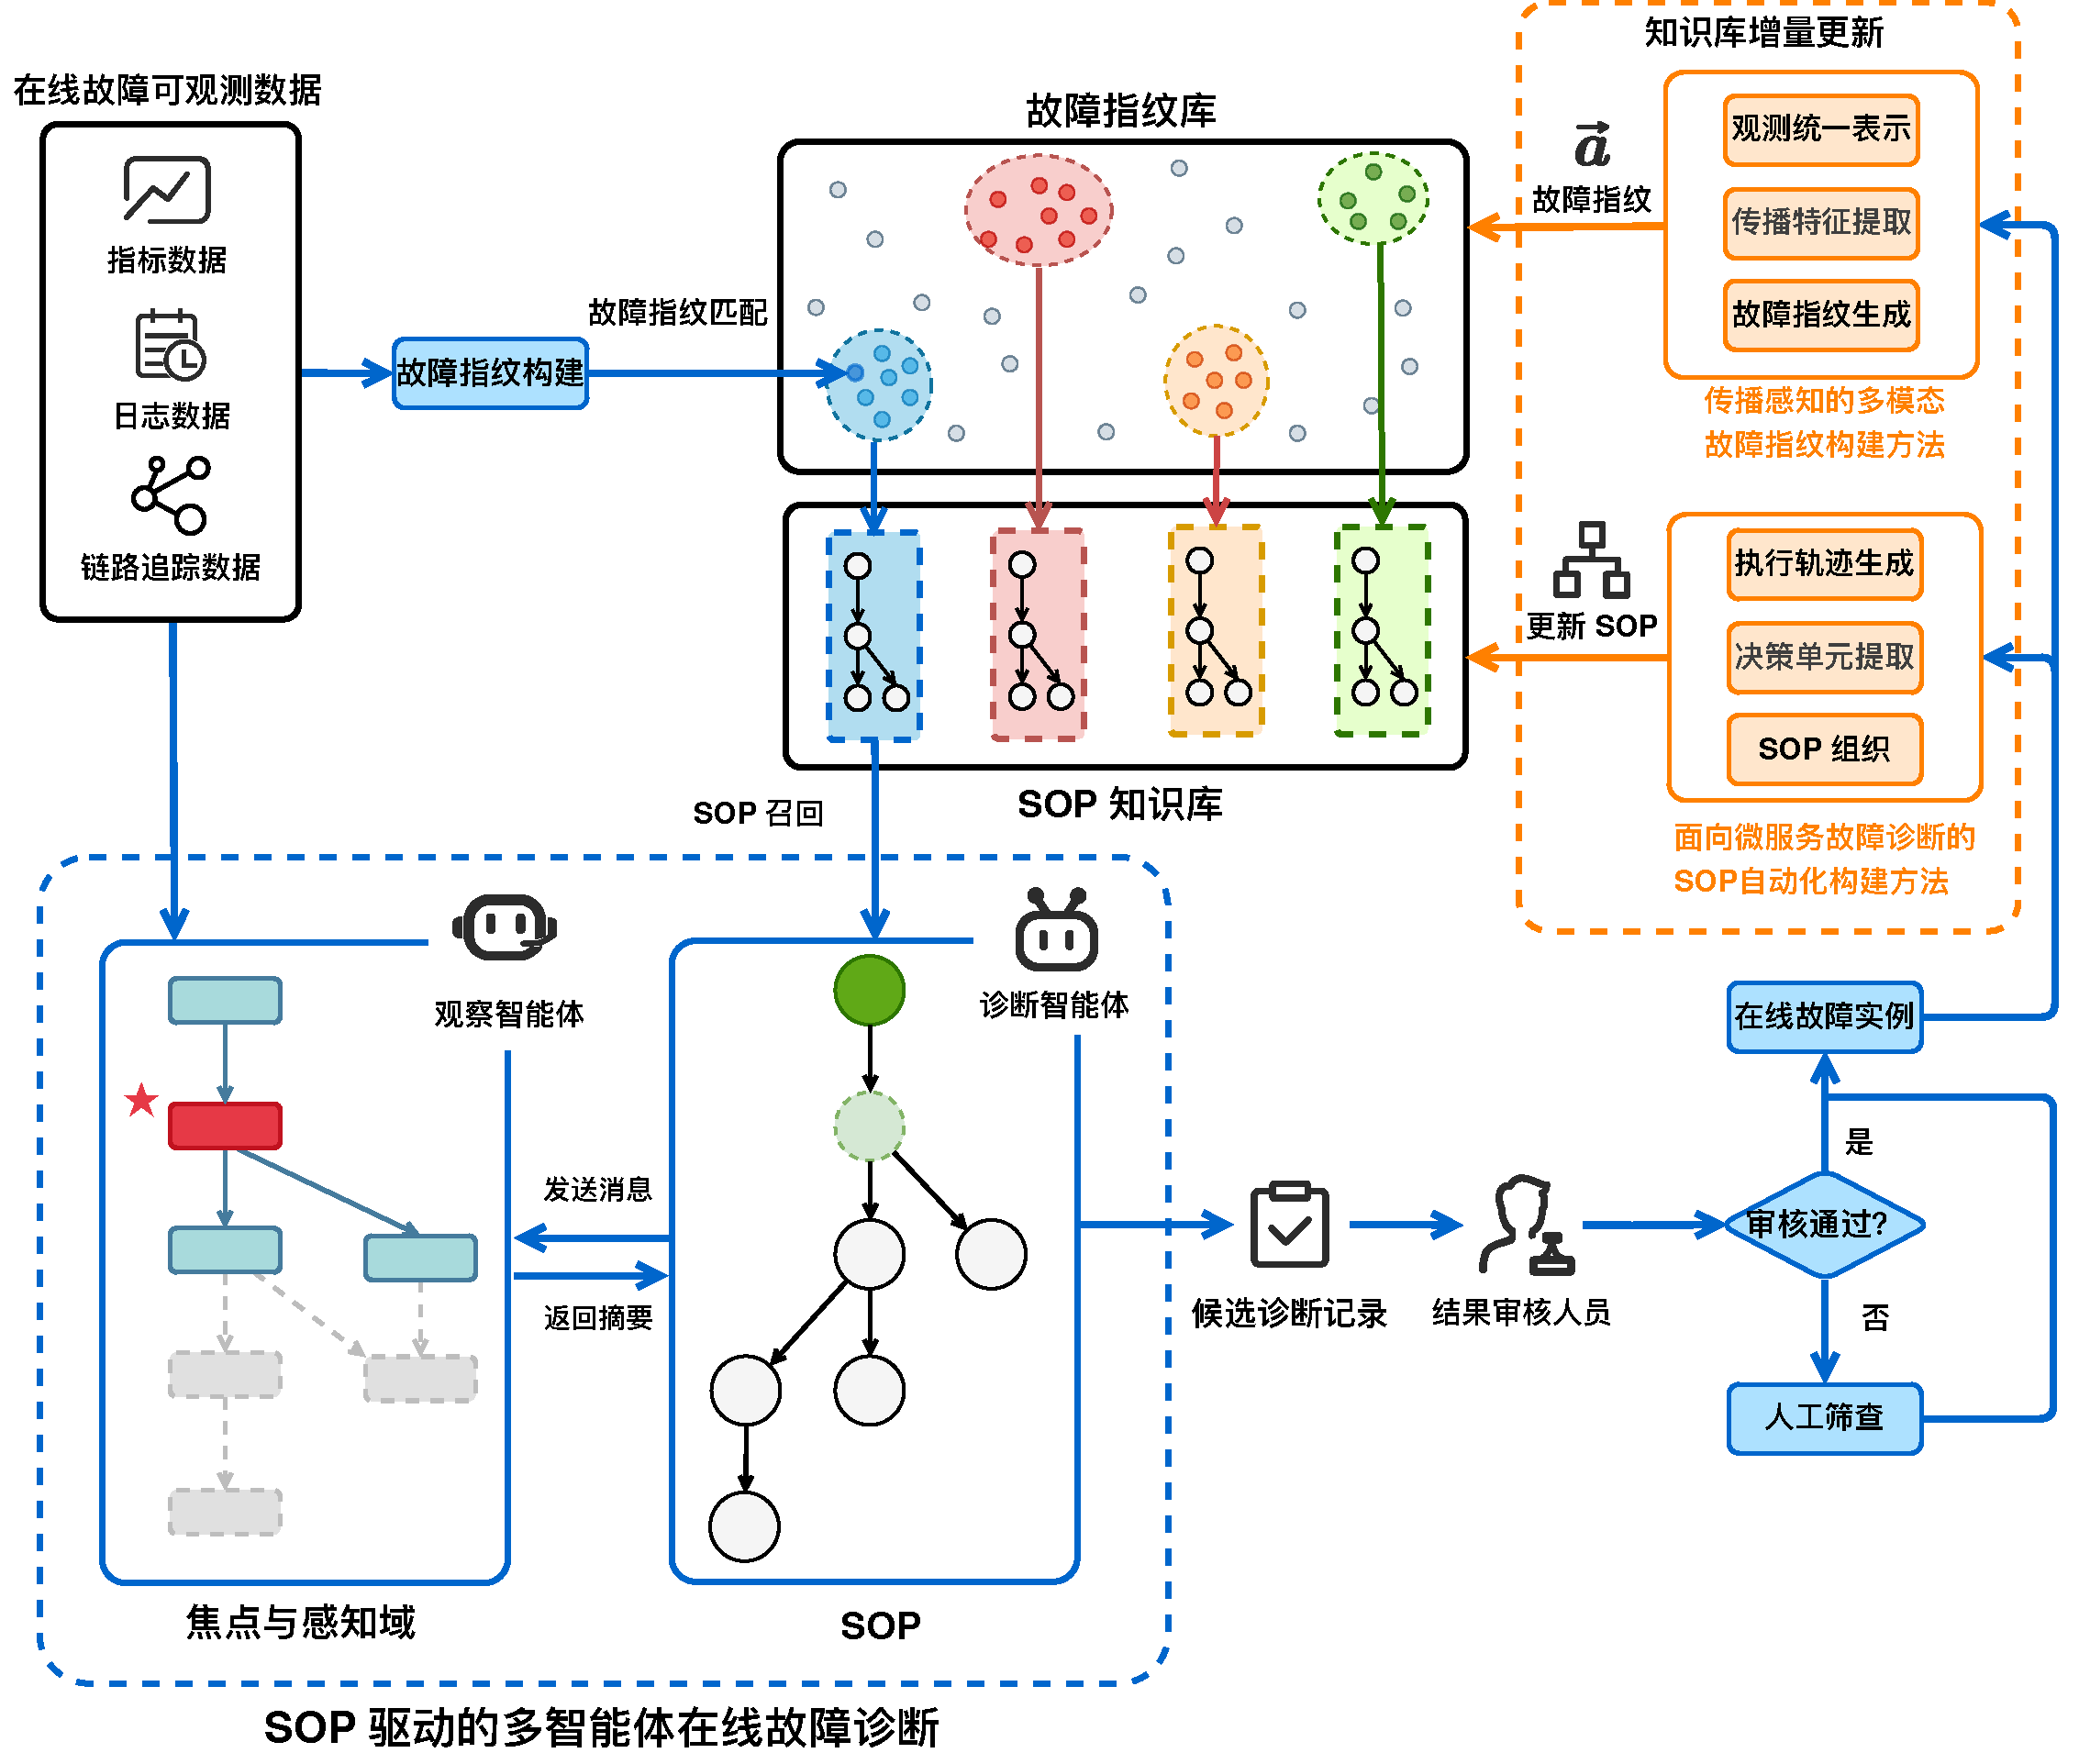
\includegraphics[width=0.8\textwidth]{Figures-Src/Chap3-Methodology/online-diagnosis-overview/chart.pdf}
    \bicaption{\enspace SOP驱动的多智能体在线故障诊断总览}{\enspace Overview of SOP-Driven Multi-Agent Online Fault Diagnosis}
    \label{fig:online_diagnosis_overview}
\end{figure}

图\ref{fig:online_diagnosis_overview}给出了SOP驱动的多智能体在线故障诊断总览。在线阶段以上两节构建的故障指纹库和 SOP 知识库为基础：当生产环境中出现新故障时，系统先根据当前故障的指标、日志和调用链路数据生成故障指纹，并在故障指纹库中检索最相似的历史故障簇，召回其绑定的 SOP 作为初始排查路径。随后，诊断智能体与观察智能体协同执行在线诊断。诊断结束后，结果经人工审核确认，作为新的在线故障实例重新进入第3.2节和第3.3节的知识构建流程。

本节其余内容按上述流程展开：3.4.1节介绍故障指纹生成与SOP召回；3.4.2节介绍焦点与感知域约束；3.4.3节介绍SOP驱动的多智能体在线诊断流程；3.4.4节介绍在线诊断结果审核与SOP增量更新。

\subsection{故障指纹匹配与 SOP 召回}

离线阶段中，系统首先按照第3.2节的方法为每个故障实例生成故障指纹向量，并在此基础上对相似故障实例进行聚类；随后，再按照第3.3节的方法为每个故障簇维护与其对应的可执行SOP。在线阶段不能将当前故障直接对应到某一条离线SOP，因为线上故障通常只与某一类历史故障相近，而不会与某个离线故障实例在服务实例、传播范围和局部现象上完全一致。例如，历史故障可能表现为“支付服务的数据库连接池耗尽”，而当前故障则可能表现为“订单服务的数据库连接池耗尽”。二者虽然属于同类故障，但涉及的组件实例和传播路径并不相同；若直接匹配单个历史故障实例，就容易将某次离线试验中的局部细节误当作当前场景中的通用排查路径，从而影响SOP的可执行性。因此，本文将SOP绑定到故障簇，而不是绑定到某个单独的故障实例，如图\ref{fig:fingerprint_sop_binding}所示。采用按故障簇召回SOP的方式，可以保留同类故障中稳定出现的排查步骤，减弱个别实例差异对在线诊断的影响。

\begin{figure}[htbp]
    \centering
    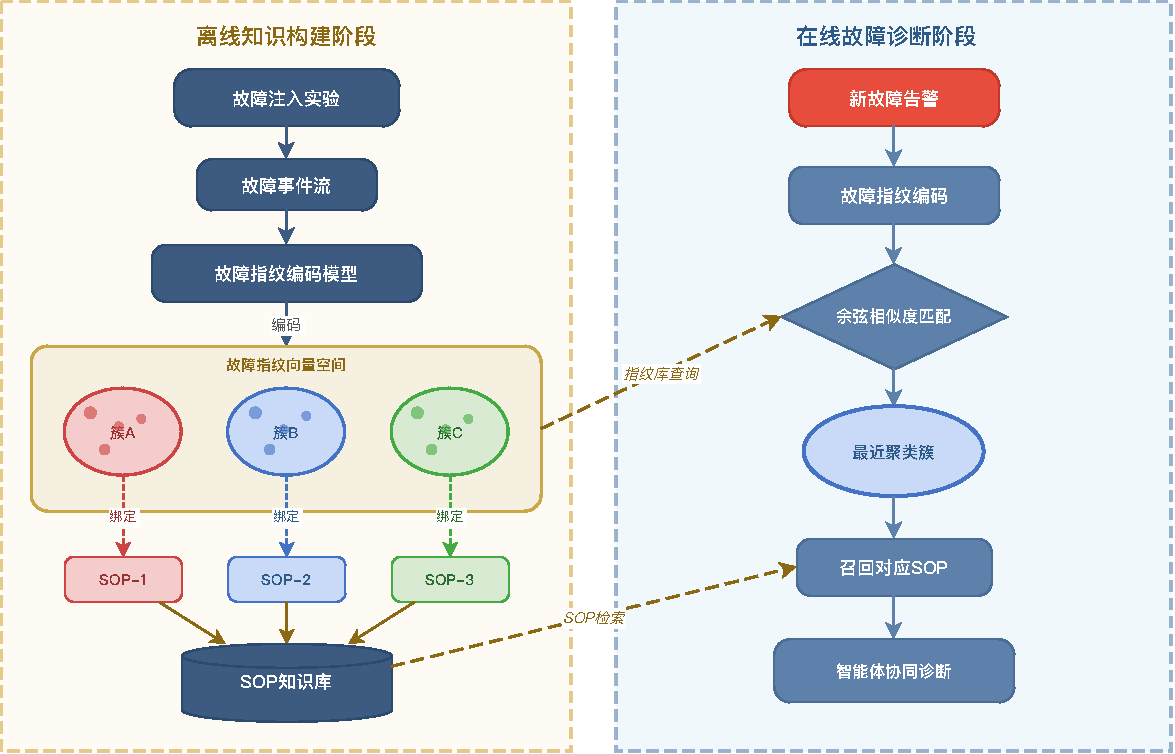
\includegraphics[width=\textwidth]{Figures-Src/Chap3-Methodology/fingerprint-sop-binding/chart.pdf}
    \bicaption{\enspace 故障指纹聚类、SOP绑定与在线召回}{\enspace Fault Fingerprint Clustering, SOP Binding, and Online Recall}
    \label{fig:fingerprint_sop_binding}
\end{figure}

对于每个故障簇，系统保存其中心向量 $\mathbf{c}_i$ 及对应的SOP。在线阶段接收新故障告警后，首先从当前故障的可观测数据中提取异常事件，并通过第3.2节中的故障指纹构建方法生成当前故障向量 $\mathbf{v}_{\text{fault}}$；随后，计算该向量与各故障簇中心向量之间的余弦相似度，并选择最相似的故障簇所绑定的SOP作为当前故障的初始排查路径：
\begin{equation}
\text{SOP}_{\text{selected}}=\arg\max_i \frac{\mathbf{v}_{\text{fault}}\cdot \mathbf{c}_i}{\|\mathbf{v}_{\text{fault}}\|\|\mathbf{c}_i\|}.
\end{equation}

完成SOP召回后，系统将诊断智能体初始化至 $\text{SOP}_{\text{selected}}$ 的入口节点，使其能够从召回的排查起点开始组织后续诊断过程。至此，系统完成了从当前故障观测数据到初始 SOP 的映射，并为后续受约束在线诊断提供了流程基础。

\subsection{焦点与感知域约束}

在前文第3.3节介绍的探索智能体基于 SOP 的探索任务执行中，探索智能体需要围绕当前任务逐步组织观察与判断，观察智能体负责返回局部证据。进一步地，在微服务场景中，服务、容器和物理节点等 K8s 层组件数量多、系统拓扑复杂；若在单轮中向诊断智能体提供过大范围的组件拓扑及其可观测数据，容易因上下文过载导致判断失稳。因此，本文在在线阶段引入焦点（Focus）与感知域（Perception Field）两个状态约束。

设第 $x$ 轮中由探索智能体指定的目标组件为焦点 $f^{(x)}$。感知域记为 $\Omega^{(x)}$，表示系统在第 $x$ 轮动态维护的组件集合。首次进入在线流程时，系统依据当前告警与可观测数据初始化初始焦点，并据此生成第一轮感知域。对于任一焦点 $f^{(x)}$，其 $k$ 跳邻域定义为
\begin{equation}
\Theta_k(f^{(x)})=\{u \mid \text{dist}_{\text{topo}}(u,f^{(x)})\leq k\},
\end{equation}
其中 $\text{dist}_{\text{topo}}(\cdot,\cdot)$ 表示系统拓扑中的结构距离，$k$ 表示感知域半径。这里的 $\Theta_k(f^{(x)})$ 表示当前焦点对应的局部邻域，而感知域本身则由系统按轮次持续维护。

在后续分析过程中，探索智能体只能从当前感知域内选择新的焦点；当焦点变化后，系统会按并集式方式更新感知域。记第 $x$ 轮感知域为 $\Omega^{(x)}$，则其更新关系可以表示为
\begin{equation}
\Omega^{(x)}=\Omega^{(x-1)}\cup \Theta_k(f^{(x)}).
\end{equation}
这意味着第 $x$ 轮感知域由上一轮感知域与第 $x$ 轮焦点的 $k$ 跳邻域共同构成。因而，当焦点从当前组件转向其 $k$ 跳范围内的其他组件时，系统会将新焦点相关的服务、容器和物理节点并入当前感知域，使感知范围沿分析路径逐步展开，避免一次性引入全局拓扑信息。

\begin{figure}[htbp]
    \centering
    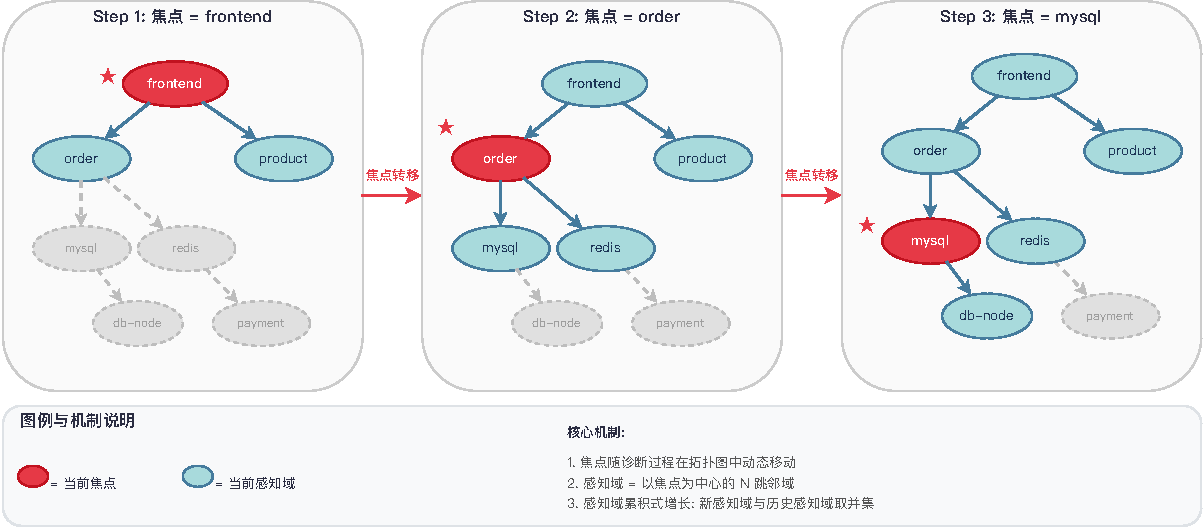
\includegraphics[width=\textwidth]{Figures-Src/Chap3-Methodology/focus-mechanism/chart.pdf}
    \bicaption{\enspace 焦点迁移与感知域变化示意}{\enspace Focus Shift and Perception Field Update}
    \label{fig:focus_mechanism}
\end{figure}

在上述机制下，观察智能体只能访问当前感知域内组件的指标、日志和链路数据，探索智能体也只能在当前感知域内切换分析对象，并可通过 \texttt{query\_status} 获取当前焦点与感知域状态。图\ref{fig:focus_mechanism}展示了焦点在系统拓扑中的迁移方式，以及感知域如何随着焦点变化而同步更新。例如，当当前焦点由支付服务切换为其数据库依赖链路上的某个组件时，系统会将该新焦点 $k$ 跳范围内相关的服务、容器和物理节点并入当前感知域；随后的观察与判断仍只在更新后的感知域内推进。通过这种方式，排查过程始终沿与当前路径直接相关的拓扑范围展开，从而兼顾在线执行效率与证据收集的有效性。

\subsection{SOP 驱动的多智能体在线诊断流程}

第3.4.2节从探索智能体与观察智能体的协同方式中抽象出了焦点与感知域这两个状态约束。进入在线阶段后，该约束由诊断智能体继承和执行。在完成故障指纹生成、SOP召回以及焦点与感知域初始化后，系统进入SOP驱动的在线诊断阶段。该阶段仍由诊断智能体与观察智能体协同完成，其运行方式在交互形式上与第3.3节中的离线探索过程相近：诊断智能体沿当前SOP节点逐步推进排查，观察智能体根据请求返回对应的指标、日志和链路证据，二者通过多轮交互不断缩小可疑范围。不同之处在于，第3.3节中的探索智能体服务于离线知识构建，其目标是在已知故障类型的前提下生成可用于构建SOP的执行轨迹；而本节中的诊断智能体服务于在线故障定位，其目标是利用召回的SOP，对当前故障逐步完成根因判断。

两类智能体虽然都与观察智能体配合完成任务，但它们分属不同阶段，面对的任务输入、输出结果以及对SOP的作用并不相同。表\ref{tab:exploration_vs_diagnosis}对这一差异作了简要对比。

\begin{table}[tbp]
    \centering
    \bicaption{\enspace 离线探索智能体与在线诊断智能体的角色差异}{\enspace Role Differences Between the Offline Exploration Agent and the Online Diagnosis Agent}
    \label{tab:exploration_vs_diagnosis}
    \renewcommand{\arraystretch}{1.2}
    \fontsize{10pt}{12pt}\selectfont
    \setlength{\tabcolsep}{4pt}
    \begin{tabular*}{\textwidth}{@{\extracolsep{\fill}}>{\centering\arraybackslash}p{2.0cm}>{\raggedright\arraybackslash}p{5.1cm}>{\raggedright\arraybackslash}p{5.1cm}@{}}
        \toprule
        \rowcolor{lightgray!30}
        \textbf{比较维度} & \textbf{探索智能体（离线）} & \textbf{诊断智能体（在线）} \\
        \midrule
        所属阶段 & 离线知识构建阶段 & 在线故障诊断阶段 \\
        \midrule
        任务前提 & 已知故障类型先验，不可见真实故障位置 & 仅有当前故障观测数据，由故障指纹召回初始 SOP \\
        \midrule
        核心职责 & 围绕可疑组件、传播路径与竞争候选展开探索，生成完整排查轨迹 & 围绕当前 SOP 节点收集证据、判断条件并逐步收敛根因 \\
        \midrule
        与 SOP 的关系 & 在当前 SOP 上导航或逃逸扩展，为 SOP 构建与修订提供依据 & 以召回 SOP 为执行约束，必要时触发逃逸机制扩展诊断路径 \\
        \midrule
        输出结果 & 带标签的 SOP执行轨迹 & 根因诊断结论及其证据链 \\
        \midrule
        对知识库的作用 & 直接作为决策单元提取与 RuleAgent 更新的输入 & 经人工审核后补全为新故障实例，触发故障指纹与 SOP 增量更新 \\
        \bottomrule
    \end{tabular*}
    \setlength{\tabcolsep}{6pt}
\end{table}

与离线探索不同，在线诊断开始时，系统输入只有当前故障的指标、日志和调用链路数据。故障指纹召回返回的是一个可作为起点的 SOP，而不是最终答案。诊断智能体仍需结合观察智能体返回的证据，持续判断当前节点对应的诊断假设是否得到支持、是否需要沿现有分支继续排查、是否应切换到其他节点，或者是否需要在当前 SOP 无法解释现象时触发逃逸机制。在线阶段的重点在于利用已有 SOP 尽快使诊断过程收敛到可信的诊断结论。

具体而言，在线诊断过程同时受到当前 SOP 节点、当前焦点和已收集证据三项信息的共同约束。当前 SOP 节点给出此时应执行的检查任务，当前焦点限定此时优先排查的组件实例，观察智能体返回的证据则用于判断当前节点对应的验证条件是否满足，以及后续应继续沿现有 SOP 推进、在 SOP 内切换分支，还是触发逃逸机制扩展新的排查路径。为便于说明，本文将 SOP 驱动的在线诊断过程概括为以下四类关键操作：

\begin{enumerate}[label=（\arabic*）]
    \item \textbf{证据收集与更新。}
    当诊断智能体到达某一 SOP 节点后，首先根据该节点对应的诊断意图、当前焦点以及已有证据，确定本轮需要观察的组件对象与证据类型，并向观察智能体发出诊断请求。观察智能体随后在当前感知域内收集相应的指标、日志和调用链路数据，并将其整理为可供后续判断的结构化证据。随着新证据不断加入，系统对当前故障状态的刻画也随之更新，为后续路径判断提供依据。

    \item \textbf{SOP 内分支导航。}
    若新收集到的证据尚不足以支持沿当前节点的主分支继续推进，但已能够表明当前检查方向不成立，且现有 SOP 中仍存在其他可供验证的分支，则诊断智能体不会立即脱离当前 SOP，而是在当前 SOP 内转向其他候选检查路径。此时，系统仍保持当前感知域约束，仅在已有 SOP 覆盖的范围内调整排查方向，从而优先利用已沉淀的诊断知识完成进一步定位。

    \item \textbf{条件满足后的节点转移。}
    若当前证据能够支持某一分支条件成立，则诊断智能体沿满足条件的边转移到下一节点，并据此更新当前检查任务与焦点位置。节点转移意味着诊断过程在现有 SOP 上取得了进一步收敛：系统不再停留于当前局部判断，而是将排查推进到下一步更具体的验证环节。随着节点不断转移，诊断过程逐步缩小可疑范围，并向最终根因结论逼近。

    \item \textbf{逃逸机制触发。}
    若当前 SOP 中不存在与现有证据相匹配的后续分支，或者在当前局部范围内持续收集证据后仍无法形成有效判断，则说明现有 SOP 尚不足以覆盖当前故障场景。此时，系统触发逃逸机制，在当前路径基础上扩展新的排查方向，并围绕新的候选对象继续收集证据与推进判断。逃逸并不意味着放弃 SOP，而是在既有知识无法解释当前现象时，对未被覆盖的诊断路径进行补充性探索，以避免诊断过程停滞在现有结构边界处。
\end{enumerate}

在上述四类操作的交替推进下，诊断智能体与观察智能体通过多轮协同不断缩小可疑范围，并最终形成针对当前故障的诊断结果。在线诊断结束后，诊断智能体提交候选故障位置、候选故障类型及其对应的关键证据链，作为后续人工审核与知识库增量更新的输入。

\subsection{在线诊断结果审核与知识库增量更新}

在线诊断阶段的直接输出，是由诊断智能体在完成排查后提交的诊断结果，其中包含候选故障位置、候选故障类型以及支撑这些判断的证据链。该结果不宜在未经审核的情况下直接纳入知识库，因为线上故障的故障位置和故障类型需要在排查过程中逐步判断，仍可能存在误判。例如，系统诊断智能体可能将故障诊断为“数据库连接池耗尽”，但实际处置后发现根因是“慢查询导致连接堆积”。如果不经过人工审核就直接更新知识库，就会将错误案例引入历史故障数据，进而影响后续故障指纹召回与 SOP执行效果。

因此，诊断结果仍需由人工结合实际处置过程、业务恢复情况、组件修复记录以及必要的事后分析进行审核。只有当人工审核确认该结果与实际处置情况一致后，它才会被确认为新的在线故障实例。经确认后的在线故障实例会重新进入前两节给出的知识沉淀过程：一方面，系统按照第3.2节的方法为该实例生成故障指纹，并判断其应归入现有故障簇还是形成新的故障簇，从而更新故障指纹库及其聚类结果；另一方面，系统按照第3.3节的方法围绕该实例补充 SOP执行轨迹，提取新的决策单元并计算权重，再基于规则对现有 SOP 进行增量修订。这样可以避免把单次在线结论中的偶然现象或临时处置动作直接固化为通用流程。
